% 2007 年新课标卷理科第 20 题：正方形 ABCD 内的不规则图形 M。
% 来源 PDF：gaokaomath-src/普通高考/2007/2007新课标理(海南,宁夏).pdf
% SHA-256：c8ee1632ac3a7a28aab1150f047a2e1c74398ca2944701e9165237897ae724e2
% 原页：2007新课标理(海南,宁夏).pdf 第 2 页（A3 三栏）第 1 栏，书页码 394。
% 重绘依据：按原页正方形的顶点标注与内部不规则阴影轮廓重绘，轮廓为示意。
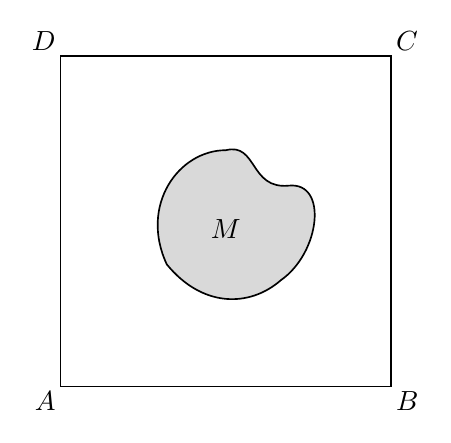
\begin{tikzpicture}[scale=1.0, semithick,
  every node/.style={inner sep=1.5pt}]

  \draw (0,0) rectangle (4.2,4.2);
  \node[below left] at (0,0) {$A$};
  \node[below right] at (4.2,0) {$B$};
  \node[above right] at (4.2,4.2) {$C$};
  \node[above left] at (0,4.2) {$D$};

  \fill[gray!30]
    (1.35,1.55) .. controls (1.0,2.3) and (1.5,3.0) ..
    (2.1,3.0) .. controls (2.5,3.1) and (2.4,2.5) ..
    (2.9,2.55) .. controls (3.4,2.6) and (3.3,1.7) ..
    (2.8,1.35) .. controls (2.4,1.0) and (1.8,1.0) ..
    (1.35,1.55) -- cycle;
  \draw
    (1.35,1.55) .. controls (1.0,2.3) and (1.5,3.0) ..
    (2.1,3.0) .. controls (2.5,3.1) and (2.4,2.5) ..
    (2.9,2.55) .. controls (3.4,2.6) and (3.3,1.7) ..
    (2.8,1.35) .. controls (2.4,1.0) and (1.8,1.0) ..
    (1.35,1.55) -- cycle;
  \node at (2.1,2.0) {$M$};
\end{tikzpicture}
